\newpage
\section{Model Comparisons}
In this final section, we will compare the three models discussed in this thesis, analyzing their training phases, performance during testing phase, and identifying their strengths and weaknesses through the previous evaluation phase. We will determine which of these models is more suitable for solving the problem of time series imputation of photovoltaic data. It's essential to specify that to perform these comparisons, we reran the evaluation phase, fixing the gap size at 2 days and recalculating the various metrics used.

%In questa ultima sezione andremo a confrontare i tre modelli discussi in questa tesi, mettendo a confronto le loro fasi di training, performance ottenute durante la fase di testing, pregi e difetti individuati tramite la precedente fase di valutazione. Andremo quindi a vedere quale tra questi risulterà essere più adatto
%alla risoluzione del problema dell'imputazione di serie temporali di dati fotovoltaici. E' importante specificare che per effettuare questi confronti è
%stata rieseguita la fase di valutazione fissando la gap size a 2 giorni e ricalcolando le varie metriche impiegate.
%

\begin{table}[H]
	\centering
	\begin{tabular}{l|c|c|c|c}
		             &
		\makecell{\textbf{Model Size}                                   \\\textbf{(KB)}}
		             & \makecell{\textbf{Train Time}                    \\\textbf{(s)}}&
		\makecell{\textbf{GPU Usage}                                    \\\textbf{(\%)}} &
		\makecell{\textbf{CPU Usage}                                    \\\textbf{(\%)}}\\
		\hline
		\textbf{MLP} & 101.30                        & 24.00  & 20 & 10 \\
		\textbf{RNN} & 366.60                        & 49.00  & 20 & 27 \\
		\textbf{TRN} & 2400.0                        & 900.00 & 96 & 56
	\end{tabular}
	\caption{The table presents some data obtained during the training phase of each model.}
	%Nella tabella sono riportiati alcuni dati ottenuti durante la fase di addestramento di ogni modello.}
	\label{tab:cmptrainphase}
\end{table}

Analyzing the data shown in Table~\ref{tab:cmptrainphase}, we can see that the fastest and lightest model to train is the MLP-based one, followed by the RNN-based architecture, and finally, the Transformer. As seen in the previous sections, the first two models can certainly be trained on less powerful hardware compared to the available one, while it might be challenging for the last model. However, it's important to note that the inference time for each model is less than a second.

For all three models, the training phase was successfully completed without encountering significant issues. Comparing the graphs showing the training and validation loss curves, as shown in Figure~\ref{fig:ufcntraining}, \ref{fig:grruntraining}, and \ref{fig:gabtrainchart}, we can see that the best one is the Transformer-based model with a final validation loss value of 0.02, which is 0.01 lower than that of the RNN-based model.
%Analizzando i dati mostrati nella Tabella~\ref{tab:cmptrainphase} possiamo vedere che il modello più leggero e veloce ad addestrare risulta essere quello basato su MLP, segito poi dall'architettura che sfrutta le RNN ed infine il Transformer. Come anche visto nelle precedenti sezioni, i primi due modelli potrebbero essere sicuramente addestrati anche su architetture meno perfomanti di quella a nostra disposizione, mentre per l'ultimo probabilmente potrebbe essere molto difficile. Ricordiamo però che il tempo di inferenza per ognuno risulta essere inferiore al secondo di tempo.

%Per tutti e tre i modelli la fase di training è conclusa con successo senza riscontrare particolari problematiche. Confrontando i grafici che mostrano le curve della training e validation loss, riportati in Figura~\ref{fig:ufcntraining}, \ref{fig:grruntraining} e \ref{fig:gabtrainchart}, possiamo vedere come la migliore risulta essere quella del modello basato su Transformer con un valore finale della validatin loss di 0.02, inferiore di 0.01 rispetto a quella del modello basato su RNN.

\begin{table}[H]
	\centering
	\begin{tabular}{l|c|c|c|c|c}

		                   & \textbf{MLP}    & \textbf{RNN}    & \textbf{TRN}   & \multicolumn{2}{c}{\textbf{Incr. Gain (\%)}}         \\
		%\textbf{Model} & \textbf{MAE (kW)} & \textbf{MAPE (\%)} & \textbf{R$^2$} \\
		\hline
		                   &                 &                 &                & RNN                                          & TRN   \\
		\cline{5-6}
		\textbf{MAE (kW)}  & 14.11$\pm$3.81  & 6.86$\pm$1.87   & 3.76$\pm 0.39$ & 51.38                                        & 45.18 \\
		\textbf{MAPE (\%)} & 70.98$\pm$27.99 & 28.83$\pm$10.02 & 18.14$\pm$6.76 & 59.38                                        & 30.07 \\
		\textbf{R$^2$}     & 0.69$\pm$0.17   & 0.92$\pm$0.06   & 0.98$\pm$0.02  & 25.00                                        & 6.12

		%MAE (kW) & 14.11$\pm$3.81 & 70.98$\pm$27.99 & 0.69$\pm$0.17\\
		%MAPE (\%) &6.86$\pm$1.87 &28.83$\pm$10.02 &0.92$\pm$0.06\\
		%R$^2$ & 3.76$\pm 0.39$ &18.14$\pm$6.76 & 0.98$\pm$0.02
	\end{tabular}
	\caption{In the table, you can find the average values of MAE, MAPE, and the $R^2$ index for the three models, along with their respective standard deviations. Additionally, the Incremental Gain is provided, showing the percentage increase of the RNN model compared to MLP and the Transformer compared to RNN.}
	%Nella tabella sono riportati i valori medi del MAE, MAPE e indice $R^2$ dei tre modelli con la relativa deviazione standard. Viene inoltre mostrato l'Incremental Gain che riporta l'incremento in percentuale del modello RNN confronto al MLP e del Transformer confronto l'RNN.}
	\label{tab:comglobalmetrics3modelli}
\end{table}


\begin{figure}[H]
	\centering
	\begin{subfigure}{\textwidth}
		\centering
		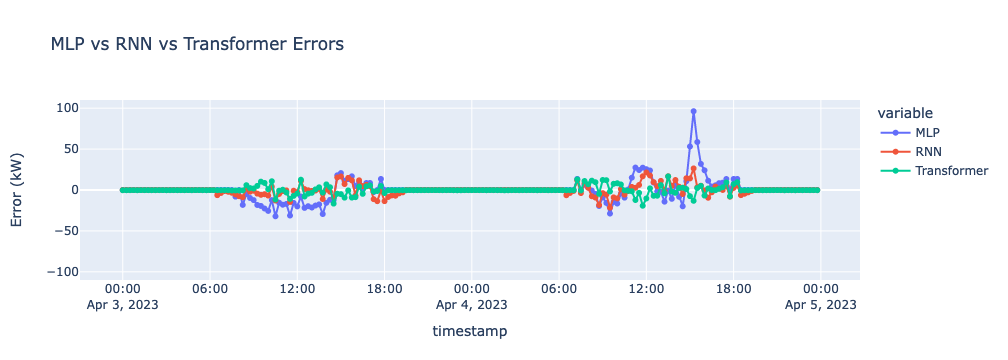
\includegraphics[width=\textwidth]{chapters/4_evaluation/imgs/cmp1.png}
		\caption{}
	\end{subfigure}
	%\begin{subfigure}{\textwidth}
	%    \centering    
	%    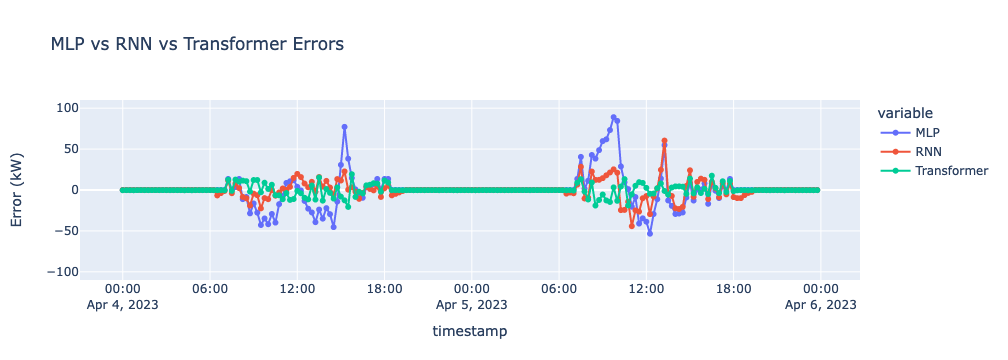
\includegraphics[width=.85\textwidth]{chapters/4_evaluation/imgs/cmp2.png}
	%    \caption{}
	%\end{subfigure}
	\begin{subfigure}{\textwidth}
		\centering
		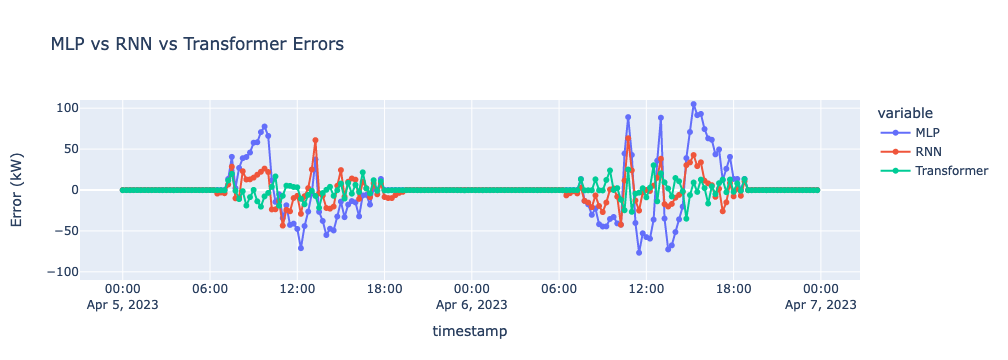
\includegraphics[width=\textwidth]{chapters/4_evaluation/imgs/cmp3.png}
		\caption{}
	\end{subfigure}
	\begin{subfigure}{\textwidth}
		\centering
		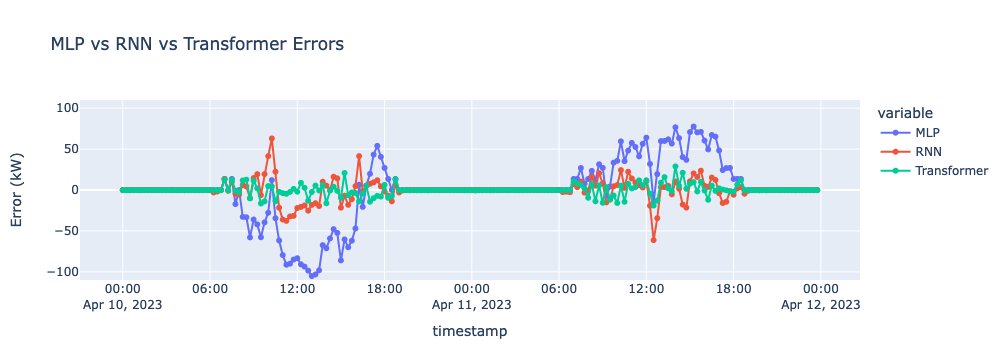
\includegraphics[width=\textwidth]{chapters/4_evaluation/imgs/cmp4.png}
		\caption{}
	\end{subfigure}
	\caption{The figure compares the errors made by the three models in predicting gaps with a two-day gap size. The blue curve represents the errors of the MLP-based model, the red curve represents the errors of the RNN-based model, and the green curve represents the errors of the Transformer-based model.}
	%Nella figura vengono paragonati gli errori commessi dai tre modelli nella predizione di buchi con gap size pari a due giorni. La curva in blu mostra gli errori commessi dal modello basato su MLP, la curva rossa fa riferimento agli errori del modello basato su RNN e quella verde del modello basato su Transformer.}
	%Nella figura sono mostrati alcuni risultati del modello ottenuti durante la fase di testing, utilizzando gap size di lunghezza variabile. Possiamo vedere gli output del modello (in rosso) confrontati con le relative ground truth (in blu).}
	\label{fig:cmperrs}
\end{figure}

Examining Table~\ref{tab:comglobalmetrics3modelli}, which shows the average values of MAE, MAPE, and the $R^2$ index for the various models, we can observe that the one based on the Transformer is significantly better. The RNN-based model is undoubtedly better than the MLP-based one, with the MAE value being 51\% lower and the MAPE showing an improvement of almost 60\%. The $R^2$ index has also improved by 25\%, indicating that the output of this model much better approximates the instantaneous energy values produced by the plant during 2-day gap periods.

However, the Transformer-based architecture excels in this task, with a 45\% improvement in MAE compared to the RNN-based model, a 30\% improvement in MAPE, and a 6\% improvement in the $R^2$ index. This model performs significantly better in predicting the plant's instantaneous energy compared to the RNN-based model, with the added capability of better detecting and understanding the presence of production peaks even over significantly variable time intervals.

%Prendendo in esame la Tabella~\ref{tab:comglobalmetrics3modelli}, dove sono riportate i valori medi di MAE, MAPE e indice $R^2$ per i vari modelli, possiamo osservare come il migliore risulta essere decisamente quello basato su Transformer.
%Il modello basato su RNN è indubbiamente migliore di quello basato su MLP, infatti il valore del MAE è inferiore del 51\%, similmente per il MAPE che abbiamo un miglioramento di quasi il 60\%. Anche l'indice $R^2$ è migliorato del 25 \% suggerendoci ce l'output di questo modello approssima nettamente meglio i valori dell'energia istantanea prodotta dall'impianto durante periodi di buchi di 2 giorni.
%
%L'architettura basata su Transformer eccelle però in questo compito avendo un MAE migliore del 45\% rispetto al modello basato su RNN, un miglioramento del 30\% sul MAPE e del 6\% sull'indice $R^2$. Questo modello riesce
%sicuramente meglio nel predirre l'energia istantanea dell'impianto rispetto all'RNN, avendo anche la capacità di individuare e comprendere molto meglio la presenza di eventuali picchi di produzione anche su intervalli di tempo notevolmente variabili.

\begin{table}[H]
	\centering
	\begin{tabular}{l|c|c|c}
		             & \textbf{AVG MAE (kW)} & \textbf{AVG Min Err (kW)} & \textbf{AVG Max Err (kW)} \\
		\hline
		\textbf{MLP} & 13.91                 & 0.35                      & 96.81                     \\
		\textbf{RNN} & 7.14                  & 0.20                      & 65.56                     \\
		\textbf{TRN} & 3.76                  & 0.12                      & 26.39
	\end{tabular}
	\caption{The table displays the average values of the metrics presented in Table~\ref{tab:cmperrtab}.}
	% Nella tabella sono riportate i valori medi delle metriche presenti nella Tabella~\ref{tab:cmperrtab}.}
	\label{tab:cmpavgdiffs}
\end{table}

These statements are supported by the graphs presented in Figure~\ref{fig:cmperrs} and the corresponding data in Tables~\ref{tab:cmperrtab} and \ref{tab:cmpavgdiffs}. The graphs illustrate the differences in point errors made by the various models. From these, we can see that the Transformer's errors (green line) are extremely compact and often close to the ideal value of 0, with an average value of 3.76 kW. The model based on RNN also has a similar curve (red line) but with values slightly farther from the ideal value and occasional error peaks, with an average value of 7.14 kW. The model based on MLP shows the worst error curve, often significantly deviating from the value of 0, featuring high error peaks, and having an average value of 13.91 kW.

We can also observe that the model based on the Transformer has a much lower average maximum point error, at 26.40 kW, compared to the RNN at 65.55 kW and the MLP at 98.81 kW. Similarly, for the average minimum point error, the Transformer-based architecture consistently performs the best, with an average value of 0.12 compared to 0.20 for RNN and 0.35 for MLP.
%Queste affermazioni vengono supportante anche dai grafici presenti in Figura~\ref{fig:cmperrs} e dai relativi dati in Tabella~\ref{tab:cmperrtab} e \ref{tab:cmpavgdiffs}.
%I primi mostrano le differenze tra gli errori puntuali commessi dai vari modelli. Da questi possiamo vedere come gli errori del Transformer (linea verde) risultano essere estremamente compatti e molto spesso vicini al valore ideale 0, con un valor medio di 3.76 kW. Anche il modello basato su RNN presenta
%una curva simile (linea rossa) ma con valore leggermente più distanti dal valore ideale con anche la presenza di qualche picco di errore e un valor medio di 7.14 kW. La curva degli errori peggiore è indubbiamente quella del modello basato su MLP che risulta molto spesso distante dal valore 0 con elevati picchi di errore e con un valore medio di 13.91 kW.
%
%Possiamo anche notare come il modello basato su Transformer ha come valor medio per il messimo errore puntuale commesso 26.40 kW decisamente molto inferiore rispetto a quello dell'RNN che è di 65.55 kW e quello dell'MLP di 98.81 kW. 
%Similmente per il minimo errore puntuale commesso dai modelli abbiamo che il migliore risulta essere sempre l'architettura basata su Transformer con un valore medio di 0.12 rispetto a quello di 0.20 e 0.35 per RNN e MLP.
%


\begin{table}[H]
	\centering
	\begin{subfigure}{\textwidth}
		\centering
		\begin{tabular}{l|l|l|l|l|l}
			\multicolumn{1}{c|}{\textbf{Gap}} & \multicolumn{3}{c|}{\textbf{MAE (kW)}}
			                                  & \multicolumn{2}{c}{\textbf{Incr. Gain (\%)}}                                                             \\
			\hline
			                                  & \textbf{MLP}                                 & \textbf{RNN} & \textbf{TRN} & \textbf{RNN} & \textbf{TRN} \\
			\cline{2-6}
			03-04 to 04-04                    & 6.90                                         & 3.65         & 2.73         & 47.10        & 25.21        \\
			04-04 to 05-04                    & 10.41                                        & 5.87         & 3.72         & 43.61        & 36.63        \\
			05-04 to 06-04                    & 17.99                                        & 7.83         & 4.25         & 56.48        & 45.72        \\
			10-04 to 11-04                    & 22.14                                        & 6.90         & 3.88         & 68.83        & 43.76
		\end{tabular}
		\caption*{(a)}
		%\vspace{1cm}
		%\caption{Nella tabella è riportato, per ogni modello, il valore del MAE (kW) nel relativo periodo in cui sono stati testati. Inoltre viene anche mostrato il valore dell' Incremental Gain in percetale del modello RNN rispetto a quello MLP e del Transformer rispetto all'RNN. Questi dati fanno riferimento ai grafici di Figure~\ref{fig:cmperrs}.}
		%\label{tab:compmae}
	\end{subfigure}
	%\vspace{1cm}
	\begin{subfigure}{\textwidth}
		\centering
		\begin{tabular}{l|l|l|l|l|l}
			\multicolumn{1}{c|}{\textbf{Gap}} & \multicolumn{3}{c|}{\textbf{Min. Err. (kW)}}
			                                  & \multicolumn{2}{c}{\textbf{Incr. Gain (\%)}}                                                             \\
			\hline
			                                  & \textbf{MLP}                                 & \textbf{RNN} & \textbf{TRN} & \textbf{RNN} & \textbf{TRN} \\
			\cline{2-6}
			03-04 to 04-04                    & 0.10                                         & 0.05         & 0.04         & 50.00        & 20.00        \\
			04-04 to 05-04                    & 0.20                                         & 0.14         & 0.05         & 30.00        & 64.28        \\
			05-04 to 06-04                    & 0.07                                         & 0.03         & 0.02         & 57.14        & 33.33        \\
			10-04 to 11-04                    & 0.19                                         & 0.13         & 0.10         & 31.57        & 23.07
		\end{tabular}
		\caption*{(b)}
	\end{subfigure}
	\begin{subfigure}{\textwidth}
		\centering
		\begin{tabular}{l|l|l|l|l|l}
			\multicolumn{1}{c|}{\textbf{Gap}} & \multicolumn{3}{c|}{\textbf{Max. Err. (kW)}}
			                                  & \multicolumn{2}{c}{\textbf{Incr. Gain (\%)}}                                                             \\
			\hline
			                                  & \textbf{MLP}                                 & \textbf{RNN} & \textbf{TRN} & \textbf{RNN} & \textbf{TRN} \\
			\cline{2-6}
			03-04 to 04-04                    & 96.28                                        & 26.38        & 19.22        & 72.60        & 27.14        \\
			04-04 to 04-05                    & 89.01                                        & 60.44        & 20.69        & 32.10        & 65.77        \\
			05-04 to 06-04                    & 105.01                                       & 63.29        & 35.10        & 39.73        & 44.54        \\
			10-04 to 11-04                    & 105.20                                       & 63.05        & 28.85        & 40.06        & 54.24
		\end{tabular}
		\caption*{(c)}
	\end{subfigure}
	\caption{In the table, the values of MAE (a), Minimum Error (b), and Maximum Error (c) are reported for each model in their respective testing periods. Additionally, the Incremental Gain in percentage is also shown for the RNN compared to the MLP and the Transformer compared to the RNN. These data correspond to the graphs in Figure~\ref{fig:cmperrs}.}
	%Nelle tabella è riportato, per ogni modello, il valore del MAE (a), Minimo Errore commesso (b) e Massimo Errore commesso (c) nel relativo periodo in cui sono stati testati. Inoltre viene anche mostrato il valore dell' Incremental Gain in percetale del modello RNN rispetto a quello MLP e del Transformer rispetto all'RNN. Questi dati fanno riferimento ai grafici di Figure~\ref{fig:cmperrs}.}
	\label{tab:cmperrtab}
\end{table}

Finally, after the analysis presented in this chapter of the various models, we can conclude that the best model for solving the imputation problem with data from time series of photovoltaic plants, despite the somewhat resource-intensive training phase, is undoubtedly the one based on the Transformer. This is due to its low MAE and MAPE values, and its near-perfect $R^2$ index. Moreover, the RNN-based model performs reasonably well in this task and could be a good alternative if one is willing to accept a slightly higher overall error in exchange for a significantly faster and lighter training phase compared to the Transformer.

%Infine, dopo l'analisi riportata in questo capitolo dei vari modelli, possiamo concludere che il migliore per 
%risolvere il problema dell'imputation su dati provenienti da serie temporali di impianti fotovoltaici, nonostante la fase di training sia
%abbastanza onerosa in termini di risorse hardware, sia sicuramente quello basato su Transformer, dato il basso valore del MAE, MAPE e del quasi perfetto valore per l'indice $R^2$. Inoltre, anche il modello basato su RNN riesce abbastanza bene in questo compito e potrebbe essere una buona alternativa, se si accetta un errore generale leggermente più alto, al Transformer per la fase di addestramento notevolmente più veloce e leggera.

%\begin{table}[H]
%    \centering
%    \begin{tabular}{l|l|l|l|l|l}
%         \multicolumn{1}{c|}{\textbf{Gap}} & \multicolumn{3}{c|}{\textbf{Min. Err. (kW)}}
%         & \multicolumn{2}{c}{\textbf{Gain (\%)}}\\
%         \hline
%         & \textbf{MLP} & \textbf{RNN} & \textbf{TRN}& \textbf{RNN} & \textbf{TRN} \\
%            \cline{2-6}
%         03-04 to 04-04 & 0.10&0.05&0.04&&\\
%         04-04 to 05-04 &0.20&0.14&0.05&&\\
%         05-04 to 06-04&0.07&0.03&0.02&&\\
%         10-04 to 11-04 &0.19&0.13&0.10&&
%    \end{tabular}
%    \caption{Nella tabella è riportato, per ogni modello, il valore del Minimo Errore commesso nel relativo periodo in cui sono stati testati. Inoltre viene anche mostrato il valore dell' Incremental Gain in percetale del modello RNN rispetto a quello MLP e del Transformer rispetto all'RNN. Questi dati fanno riferimento ai grafici di Figure~\ref{fig:cmperrs}.}
%    \label{tab:compminerr}
%\end{table}
%
%\begin{table}[H]
%    \centering
%    \begin{tabular}{l|l|l|l|l|l}
%         \multicolumn{1}{c|}{\textbf{Gap}} & \multicolumn{3}{c|}{\textbf{Max. Err. (kW)}}
%         & \multicolumn{2}{c}{\textbf{Gain (\%)}}\\
%         \hline
%         & \textbf{MLP} & \textbf{RNN} & \textbf{TRN}& \textbf{RNN} & \textbf{TRN} \\
%            \cline{2-6}
%         03-04 to 04-04 & 96.28&26.38&19.22&&\\
%         04-04 to 04-05&89.01&60.44&20.69&&\\
%         05-04 to 06-04&105.01&63.29&35.10&&\\
%         10-04 to 11-04 &105.20&63.05&28.85 & &
%    \end{tabular}
%    \caption{Nella tabella è riportato, per ogni modello, il valore del Massimo Errore commesso nel relativo periodo in cui sono stati testati. Inoltre viene anche mostrato il valore dell' Incremental Gain in percetale del modello RNN rispetto a quello MLP e del Transformer rispetto all'RNN. Questi dati fanno riferimento ai grafici di Figure~\ref{fig:cmperrs}.}
%    \label{tab:compmaxerr}
%\end{table}

%We will now compare the experimental results obtained by the
%MLP and RNN-based models.
%To do this, we will retest both networks on the testing dataset,
%forcing the generation of gaps that are consistently two days
%long to facilitate comparison (see Section~\ref{sec:mlpbaseline}
%and Section~\ref{sec:rnnbasemodel}).
%We will compare their performance by calculating, for each of them,
%the pointwise error between ground truth and prediction.
%Additionally, we will compare the various other metrics used
%and discuss some strengths and weaknesses of each model.
%
%%Confronteremo ora i risultati sperimentali ottenuti
%%dai modelli basati su MLP e RNN. Per farlo andremo a testare nuovamente
%%le due reti sul dataset di testing forzando la generazione di buchi
%%sempre a 2 giorni, in modo tale da poter confrontare i risultati (vedi 
%%Sezione~\ref{sec:mlpbaseline} e \ref{sec:rnnbasemodel}). Metteremo quindi
%%a confronto le performance di questi andando a calcolare, per ognuno,
%%l'errore puntuale tra ground truth e predizione. 
%%Infine, oltre a confrontare tra di loro le altre varie metriche impiegate,
%%andremo a discutere alcuni punti di forza e debolezze di ogni modello.
%
%\begin{table}[H]
%    \centering
%    \begin{tabular}{l|l|l|l}
%    \multicolumn{1}{c}{} &
%            \multicolumn{2}{c}{\textit{lower is better}} & \\
%        \multicolumn{1}{c|}{\textbf{Gap}} &
%        \multicolumn{2}{c|}{\textbf{MAE (kW)}} &
%        \multicolumn{1}{c}{\textbf{Gain (\%)}}  \\ %% ((MLP - RNN)*100)/MLP
%        \hline
%        & \small \textbf{MLP} & \small \textbf{RNN} & \\
%        \cline{2-3}
%        02-04 to 03-04 & 18.63 & 3.91 &  79.01\\
%        03-04 to 04-04 & 06.90 & 3.29 &  52.31\\
%        04-04 to 05-04 & 10.41 & 5.55 &  46.68\\
%        05-04 to 06-06 & 17.99 & 6.89 &  61.70\\
%        06-04 to 07-04 & 20.07 & 6.78 &  66.21\\
%        07-04 to 08-04 & 14.77 & 9.25 & 37.37\\
%        08-04 to 09-04 & 15.82 & 7.85 & 50.39\\
%        09-04 to 10-04 & 10.30 & 5.82 & 43.49
%    \end{tabular}
%    \caption{This table highlights the difference between the error of the MLP-based model and the RNN-based model. The column \texttt{Gain (\%)} represents the absolute percentage difference between MLP MAE and RNN MAE.}
%    %In questa tabella viene messo in evidenza la differenza tra l'errore del modello basato su MLP e quello su Reti Ricorrenti. La colonna \texttt{Diff (kW)} è la differenza in valore assoluto tra MLP MAE e RNN MAE, mentre \texttt{Diff (\%)} è la differenza in percentuale.}
%    \label{tab:mlpvsrnndiff}
%\end{table}
%
%\begin{table}[H]
%    \begin{minipage}[t]{.45\textwidth}
%        \centering
%\begin{tabular}[t]{l|l|l|l}
%\multicolumn{1}{c}{} &
%            \multicolumn{2}{c}{\textit{lower is better}} & \\
%         \multicolumn{1}{c|}{\textbf{Gap}} &
%         \multicolumn{2}{c|}{\makecell{\textbf{Max Err.}\\\textbf{(kW)}}} & 
%         \makecell{\textbf{Gain}\\\textbf{(\%)}} \\
%         \hline
%         & \small \textbf{MLP} & \small\textbf{RNN} &\\
%         \cline{2-3}
%        02-04 to 03-04 &  90.74 & 35.74 & 60.61\\ %55.0 \\
%        03-04 to 04-04 &  96.29 & 21.69 & 77.47\\ %74.60\\
%        04-04 to 05-04 &  89.01 & 54.95 & 29.27\\ %26.06\\
%        05-04 to 06-06 &  105.01 & 53.91 & 48.66\\ %51.10\\
%        06-04 to 07-04 &  122.56 & 51.35 & 58.10\\%71.21\\
%        07-04 to 08-04 &  105.94 & 75.91 & 28.34\\ % 30.03\\
%        08-04 to 09-04 &  86.14 & 75.47 & 06.55\\%05.65\\
%        09-04 to 10-04 &  78.76 & 59.97 & 23.85%18.79
%    \end{tabular}
%    \caption*{(a)}
%    %\caption{Nella tabella viene mostrata la differenza tra i valori dell'indice $R^2$ per i due modelli.}
%    \end{minipage}%
%    \hfill
%    \begin{minipage}[t]{.45\textwidth}
%        \centering
%    \begin{tabular}[t]{l|l|l|l}
%            \multicolumn{1}{c}{} &
%            \multicolumn{2}{c}{\textit{lower is better}} & \\
%         \multicolumn{1}{c|}{\textbf{Gap}} &
%         \multicolumn{2}{c|}{\makecell{\textbf{Min Err.}\\\textbf{(kW)}}} & 
%         \makecell{\textbf{Gain}\\\textbf{(\%)}} \\
%         \hline
%         & \small \textbf{MLP} & \small\textbf{RNN} &\\
%         \cline{2-3}
%        02-04 to 03-04 & 7.58 & 0.90 & 88.12\\ %6.68 \\
%        03-04 to 04-04 & 0.79 & 0.05 & 93.67\\ %0.74 \\
%        04-04 to 05-04 & 0.39 & 0.85 & 50.11\\ %-0.46\\
%        05-04 to 06-06 & 1.45 & 0.05 & 96.55\\ %1.40 \\
%        06-04 to 07-04 & 4.84 & 0.13 & 97.31\\ %4.71 \\
%        07-04 to 08-04 & 1.73 & 1.39 & 19.65\\ %0.34 \\
%        08-04 to 09-04 & 5.19 & 0.89 & 82.85\\% 4.30\\
%        09-04 to 10-04 & 3.19 & 0.71  & 77.74\\ %2.48
%
%    \end{tabular}
%    \caption*{(b)}
%    \end{minipage}
%    \begin{minipage}{\textwidth}
%    \vspace{.1cm}
%        \centering
%    \begin{tabular}[t]{l|l|l|l}
%    \multicolumn{1}{c}{} &
%            \multicolumn{2}{c}{\textit{bigger is better}} & \\
%         \multicolumn{1}{c|}{\textbf{Gap}} &
%         \multicolumn{2}{c|}{\textbf{$R^2$}} &
%         \multicolumn{1}{c}{\textbf{Gain (\%)}} \\
%         \hline
%         & \small \textbf{MLP} & \small\textbf{RNN} &\\
%         \cline{2-3}
%        02-04 to 03-04 & 0.64 & 0.98 & 34.69\\ %-0.34\\
%        03-04 to 04-04 & 0.52 & 0.91 & 42.85\\ %-0.39\\
%        04-04 to 05-04 & 0.52 & 0.89 & 41.57\\%-0.37\\
%        05-04 to 06-06 & 0.42 & 0.91 & 53.84\\ %-0.49\\
%        06-04 to 07-04 & 0.62 & 0.95 & 37.73\\ %-0.33\\
%        07-04 to 08-04 & 0.78 & 0.91 & 14.28\\ %-0.13\\
%        08-04 to 09-04 & 0.55 & 0.85 & 35.29\\ %-0.30\\
%        09-04 to 10-04 & 0.42 & 0.78 & 46.15 %-0.36
%    \end{tabular}
%    \caption*{(c)}
%    \end{minipage}
%
%    \caption{The tables compare the results of the two models, highlighting the maximum pointwise error (a), the minimum pointwise error (b), and the $R^2$ index (c). For each metric, the absolute percentage difference is also shown.}
%    %Le tabelle mettono a confronto i risultati dei due modelli paragonando il massimo errore puntuale (a) espresso in kW, il minimo errore puntuale (b) espresso in kW e l'indice $R^2$ (c). Per ognuna viene mostrata anche la differenza tra i due valore ($MPL - RNN$).}
%\end{table}
%
%From the previous tables, it's evident that the RNN-based model achieves significantly higher $R^2$ values compared to the MLP-based model. On average, the RNN-based model's values hover around 0.90, while the MLP-based model is around 0.60, with an average difference of 30\%. The second model approximates the trend of instant energy production during gaps much better.
%
%In tables (a) and (b), it can be observed that the architecture utilizing RNN has maximum and minimum error values significantly lower than the MLP-based model. Regarding Gap MAE, the second model is also superior to the first by approximately 60\%, with significantly lower average errors.
%
%%Dalle precedenti tabelle possiamo vedere com il modello basato su RNN ottiene
%%predizioni con un indice $R^2$ molto superiore a quello del modello basato su MLP. In media i valori del primo si aggirano intorno a 0.90 mentre per 
%%il secondo siamo sul 0.60 con una differenza media di 0.30 punti. Il secondo modello approssima nettamente meglio l'andamento dell'energia istantanea prodotta durante i buchi. 
%%Dalle tabelle (a) e (b) si vede come l'architettura che sfrutta RNN 
%%ha valori di errore massimi e minimi decisamente più contenuti rispetto a quella che
%%si basa su MLP.
%%Anche per il Gap MAE possiamo vedere come il secodo modello
%%sia migliore rispetto al primo di circa il 60\% commettendo in media errori
%%nettamente più bassi rispetto all'altro.
%
%\begin{figure}[H]
%    \centering
%    \begin{subfigure}{\textwidth}
%    \centering
%    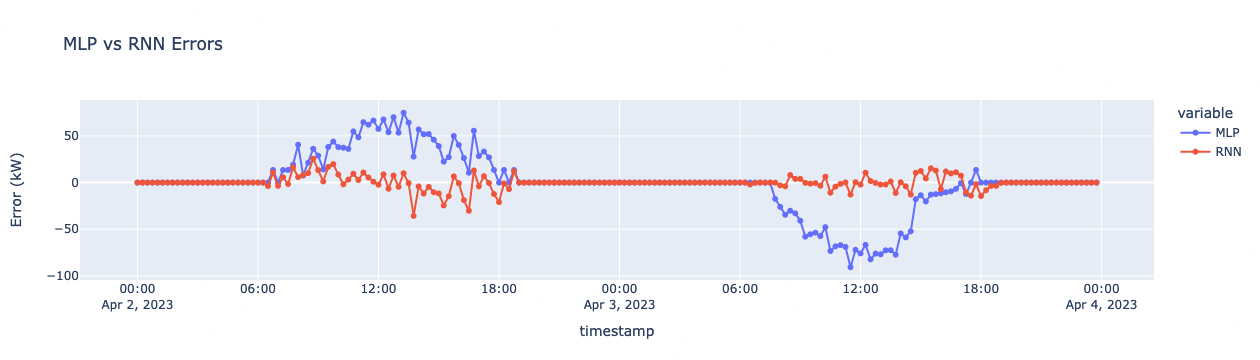
\includegraphics[width=\textwidth]{chapters/4_evaluation/imgs/mlpvsrnn/mlpvsrnn1.png}
%       \caption{} 
%    \end{subfigure}
%    \begin{subfigure}{\textwidth}
%    \centering
%    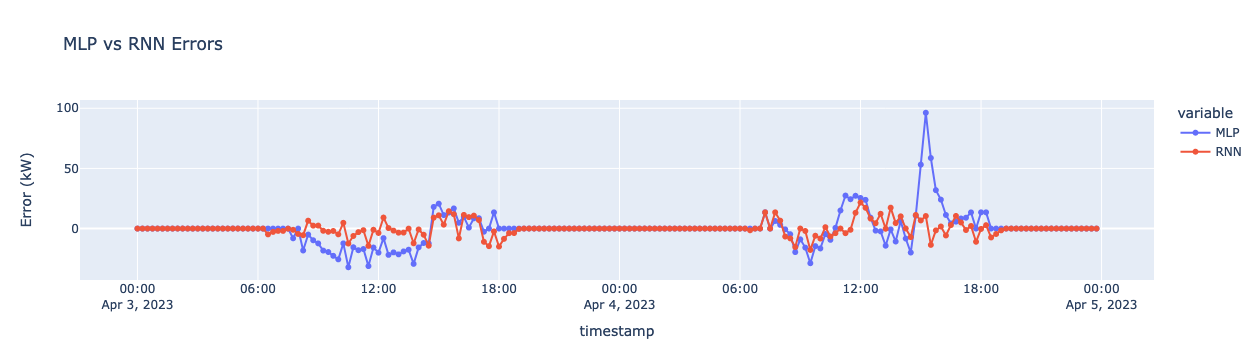
\includegraphics[width=\textwidth]{chapters/4_evaluation/imgs/mlpvsrnn/mlpvsrnn2.png}
%       \caption{} 
%    \end{subfigure}
%    \begin{subfigure}{\textwidth}
%    \centering
%    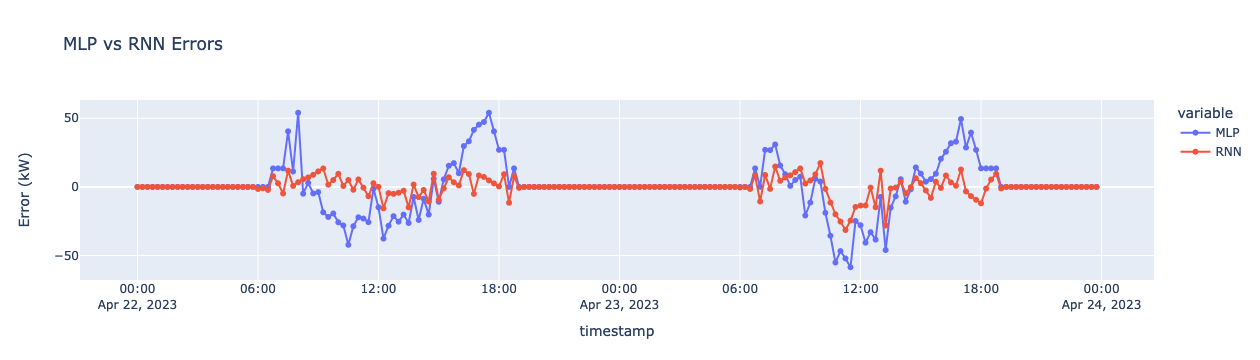
\includegraphics[width=\textwidth]{chapters/4_evaluation/imgs/mlpvsrnn/mlpvsrnn3.png}
%       \caption{} 
%    \end{subfigure}
%    \caption{The figure displays the difference curves between the target and prediction for the MLP-based models (in blue) and the RNN-based models (in red).}
%   % Nella figura sono mostrate le curve delle differenze tra target e predizione dei modelli basati su MLP (mostrate in blu) e su RNN (in rosso).}
%    \label{fig:mlpvsrnngrafici}
%\end{figure}
%From the graphs shown in Figure~\ref{fig:mlpvsrnngrafici},
%it's immediately noticeable that the architecture utilizing
%recurrent neural networks commits significantly lower errors
%than the MLP-based model.
%The red curves are generally more compact and closer to 0
%(no error committed), while the blue curves are on average
%much farther from the ideal value, indicating a significantly
%higher pointwise error, on average by 60\%, with the presence
%of substantial peaks (b).
%It's important to highlight that both models do not commit errors at night.
%
%Comparing the respective outputs of the two models,
%it's evident that the predicted curves by the MLP-based model
%are extremely similar to each other and fail to identify
%possible production peaks.
%On the other hand, the output of the second model
%performs significantly better in the task, generating curves
%that closely follow the ground truth, understanding the
%presence of potential energy peaks, and demonstrating the
%ability to generate curves with different shapes and widely
%varying values.
%
%It's also noticeable that the first model struggles with
%identifying day and night periods, often ending production a
%few hours before sunset.
%In contrast, the second model excels in understanding
%this alternation and does not exhibit issues of this nature.
%
%It's also important to note that both models are relatively
%lightweight in terms of resources for training and inference
%on the architecture at our disposal.
%This suggests the possibility of training and using
%them on less powerful machines.
%
%The second model can also close gaps of considerably larger
%sizes than those used during the training phase.
%In contrast, the first model can only handle 2-day gaps,
%and to increase this limit, the model would need to repeat
%the training phase.
%
%%Dai grafici mostrati in Figura~\ref{fig:mlpvsrnngrafici} possiamo 
%%notare immediatamente che l'architettura che sfrutta le reti ricorrenti
%%commette errori significativamente più bassi di quella basata su MLP.
%%Notiamo come le curve in rosso sono generalmente più compatte ed abbastanza
%%vicine allo 0 (nessun errore commesso). Mentre quelle in blu risultano mediamente
%%molto più distanti dal valore ideale evidenziando quindi un errore puntuale nettamente più alto, in media del 60\%, con la presenza di picchi di notevole valore (b). \'{E} importante evidenziare che di notte tutti e
%%due i modelli non commettono errori.
%
%%Confrontando i relativi output dei due modelli possiamo notare come
%%le curve predette dal modello basato su MLP siano estremamente simili
%%tra di loro e non riescono ad individuare possibili picchi di produzione.
%%Mentre l'output del secondo riesce nettamente meglio nel compito generando
%%curve che seguno bene l'andamento della ground trouth, riuscendo a comprendere
%%anche presenza di possibili picchi di energia prodotta oltre all'abilità
%%di generare curve di differente forma e valori anche moltro diversi
%%tra di loro.
%
%%Notiamo anche che il primo modello ha qualche difficoltà nel capire 
%%i periodi di giorno e notte con il risultato che molto spesso termina la 
%%produzione qualche ora prima del tramonto, mentre il secondo riesce molto
%%bene a comprendere questa alternanza e non presenta probemi di questo tipo.
%
%%\'{E} importante anche notare che tutti e due i modelli risultano relativamente
%%leggeri sia in termini di risorse per l'allenamento e per l'inferenza sull'architettura a nostra disposizione. Suggerendo quindi la possibilità
%%di essere addestrati ed usati anche su macchine meno performanti.
%
%%Il secondo modello riesce anche a chiudere buchi di dimensioni notevolmente
%%maggiori rispetto a quelli utilizzati durante la fase di training, mentre il primo riesce a gestire solo buchi di 2 giorni e per poter aumentare questo limite, il modello necessita di ripetere nuovamente la fase di trianing.
%
%\begin{figure}[H]
%    \centering
%    \begin{subfigure}{\textwidth}
%        \centering    
%        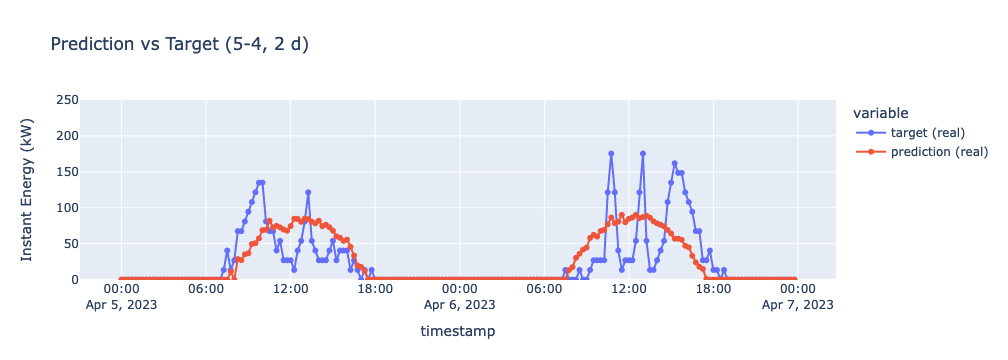
\includegraphics[width=.75\textwidth]{chapters/3_models/imgs/ufnc/eval/ufcpred5-4.png}
%        \caption{}
%    \end{subfigure}
%    \begin{subfigure}{\textwidth}
%        \centering    
%        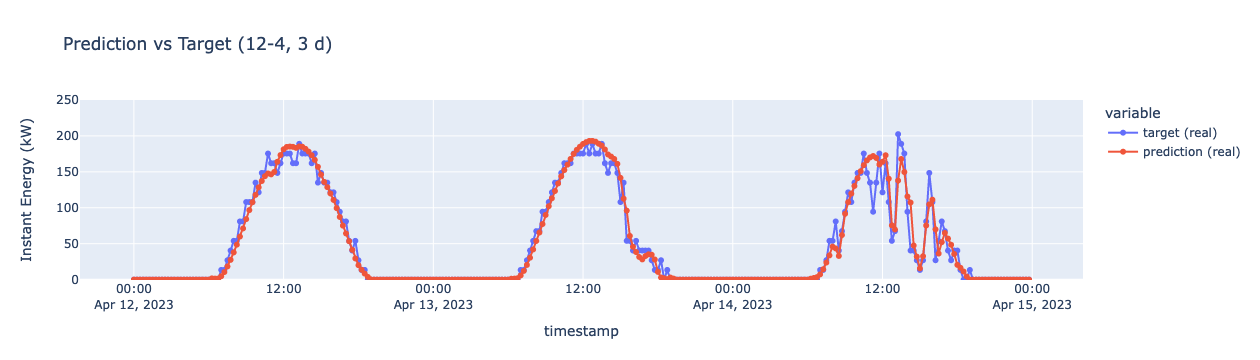
\includegraphics[width=.75\textwidth]{chapters/3_models/imgs/grrun/eval/grruneval124.png}
%        \caption{}
%    \end{subfigure}
%    \caption{Visual comparison between an output of the MLP-based model (a) and an output of the RNN-based model (b).}
%    %Confronto visuale tra un output del modello basato su MLP (a) e output del modello basato su RNN (b).}
%\end{figure}
%    